\chap{Timers and Real-time Clock}

\section{Part IV}
An early method of telegraph communication was based on the Morse code. This code uses patterns of short and long pulses to represent a message. Each letter is represented as a sequence of dots (a short pulse), and dashes (a long pulse). For example, the first eight letters of the alphabet have the following representation:
\begin{figure}[h]
    \centering
    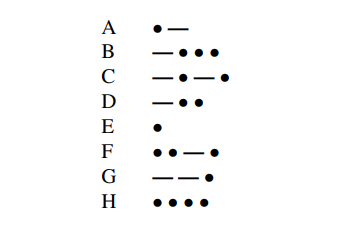
\includegraphics[scale = 0.80]{source/picture/Lab5/Lab5_1.png}
\end{figure}\\
\begin{itemize}
    \item[]\textbf{REQUIREMENT}
        \begin{enumerate}
            \item Design and implement a circuit that takes as input one of the first eight letters of the alphabet and displays the Morse code for it on a red LED.
            \item Your circuit should use switches $SW_{2-0}$ and pushbuttons $KEY_{1-0}$ as inputs. When a user presses $KEY_1$, the circuit should display the Morse code for a letter specified by $SW_{2-0}$ (000 for A, 001 for B, etc.), using 0.5-second pulses to represent dots, and 1.5-second pulses to represent dashes.
            \item Pushbutton $KEY_0$ should function as an asynchronous reset. A high-level schematic diagram of the circuit is shown in Figure 2.
                \begin{figure}[h]
                    \centering
                    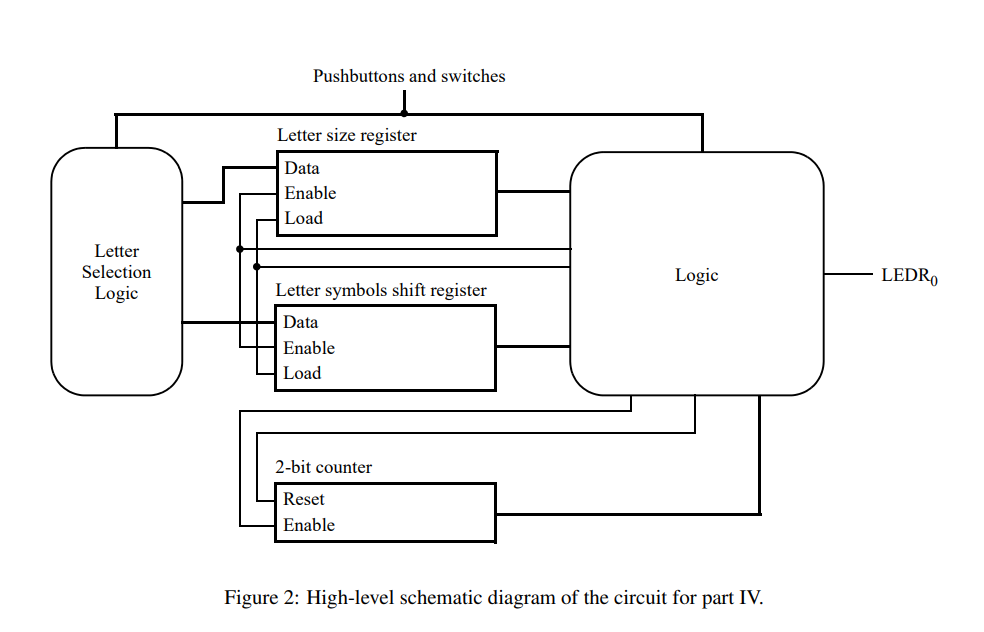
\includegraphics[scale = 0.50]{source/picture/Lab5/Lab5_2.png}
                \end{figure}
        \end{enumerate}
\clearpage
    \item[]\textbf{SOLUTION}
        \begin{itemize}
            \item [] We base on the hint given; we translate the input which has a 3-bit length into the signal 13 bits.
                \begin{lstlisting}[language = verilog]
module translate_signal(in, out);
	input		[3:0]in;
	output	reg [12:0]out;
	
	always begin
		if (in==0) out=13'b0000000111010;
		if (in==1) out=13'b0001010101110;
		if (in==2) out=13'b0101110101110;
		if (in==3) out=13'b0000010101110;
		if (in==5) out=13'b0001011101010;
		if (in==4) out=13'b0000000000010;
		if (in==6) out=13'b0001110111010;
		if (in==7) out=13'b0000010101010;
	end
endmodul
                \end{lstlisting}
            \item [] After translating, we shift left 13 times, each time, if that bit is 1 we turn on the led, if that  bit is equal to 0, we turn off the led. The period for each clock is 0.5 seconds.
                \begin{lstlisting}[language=verilog]
module part4 (CLK, RESET, EN, code, led);
	input		CLK, RESET, EN;
	input		[2:0]code;
	output	led;

	reg 		[2:0]numb;
	wire		[12:0]decode	 /*synthesis keep*/;
	wire		time_start		 /*synthesis keep*/;
	
	
	
	counter 		sub_clk 	(.CLK(CLK), .RESET(RESET), .K(25000000), .rollover(time_start), .Q());
	translate_signal	inst0 	(.in(code), .out(decode));
	defparam sub_clk.n = 25;
	
	always @(posedge time_start) numb<=numb+1;
	assign led = decode[numb] & EN;
	
				
endmodule
                \end{lstlisting}
        \end{itemize}
\end{itemize}

\clearpage
